\documentclass[12pt, a4paper]{report}
\usepackage[utf8]{inputenc}
\usepackage[T1]{fontenc}
\usepackage[margin=1in]{geometry}
\usepackage{tikz}
\usepackage{xcolor}
\usepackage[default]{tgheros} 
\usetikzlibrary{calc}
\usepackage{setspace}
\usepackage{eso-pic} % حزمة لوضع البوردر في الخلفية
\usepackage{enumitem}
\usepackage{changepage}
\usepackage{tabularx}
\usepackage{colortbl}

\definecolor{myblue}{RGB}{0, 70, 140} 

% أمر وضع البوردر في كل الصفحات
\newcommand\DrawBorder{
    \begin{tikzpicture}[remember picture, overlay]
        \draw[myblue, thick] ($(current page.north west)+(1cm,-1cm)$) rectangle ($(current page.south east)+(-1cm,1cm)$);
    \end{tikzpicture}
}
\begin{document}

% --- صفحة العنوان ---
\begin{titlepage}
    \begin{tikzpicture}[remember picture, overlay]
        \draw[myblue, thick] ($(current page.north west)+(1cm,-1cm)$) rectangle ($(current page.south east)+(-1cm,1cm)$);
    \end{tikzpicture}

    \centering
    \vspace*{3cm}
    
    % استخدام minipage للتحكم في عرض العنوان ومنع تداخله
    \begin{minipage}{1.0\textwidth}
    \centering
    \setstretch{1.3} % هذا الأمر يتحكم بالمسافة بين السطور بدقة
    {\color{myblue} \fontsize{22}{28}\selectfont \bfseries \MakeUppercase{MEDICAL DATA INTEGRATION AND INTEROPERABILITY THROUGH REMOTE MONITORING OF HEALTHCARE DEVICES USING BLOCKCHAIN}}
\end{minipage}

    
    \vspace{5cm}
    
    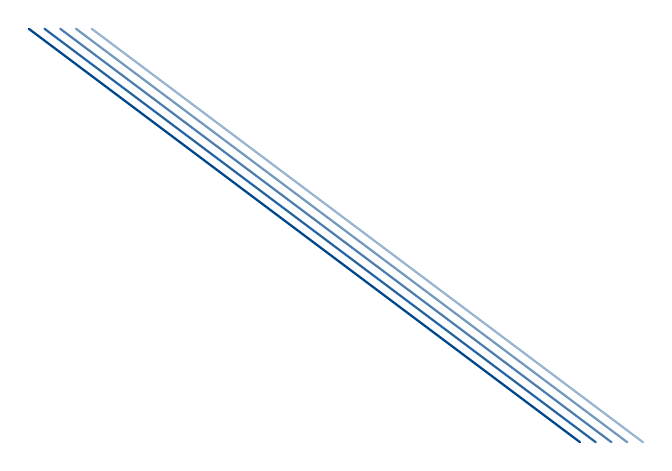
\begin{tikzpicture}[line cap=round]
        \foreach \i in {0, 1, 2, 3, 4} {
            \draw[myblue, thick, opacity={1 - (\i * 0.15)}] (\i * 0.2, 0) -- (\i * 0.2 + 7, -5.25);
        }
    \end{tikzpicture}
    
    \vfill
    
    {\color{myblue} \Large \bfseries DONE BY: ALAA KHALID}
    
    \vspace{3cm}
\end{titlepage}

\AddToShipoutPictureBG{\DrawBorder}
% --- صفحة الفصل الأول ---
\newpage

\begin{titlepage}
    \begin{tikzpicture}[remember picture, overlay]
        \draw[myblue, thick] ($(current page.north west)+(1cm,-1cm)$) rectangle ($(current page.south east)+(-1cm,1cm)$);
    \end{tikzpicture}

    \centering
    \vspace*{10cm}
    
    {\color{myblue} \fontsize{30}{36}\selectfont \bfseries CHAPTER 1}
    
    \vspace{1cm}
    
    {\color{myblue} \Huge \bfseries INTRODUCTION}
\end{titlepage}


% --- بداية صفحة المحتوى ---
\newpage
% ضبط المسافات للنص العادي
\setlength{\parskip}{1em} 

% 1.1 Background
{\color{myblue} \Large \bfseries 1.1 Background}

\noindent The emergence of IoMT at an incredible speed has revolutionized the contemporary healthcare industry, enabling real-time patient monitoring through various connected healthcare devices. Such technological innovations enable the acquisition of valuable clinical data, which significantly contributes to optimizing treatment and achieving better patient outcomes. Despite obvious benefits, the extensive deployment of heterogeneous healthcare devices has raised several challenges related to data integration and compatibility across various healthcare systems. Due to the absence of a unified approach to collecting and exchanging clinical data, information silos arise, undermining the effectiveness of diagnostic and decision-making processes. Recently, blockchain technology has emerged as a revolutionary tool capable of addressing important problems in healthcare management. Introducing an innovative blockchain-based data management model makes it possible to overcome current shortcomings in the field, including the protection and security of patient information.

\vspace{0.5cm}

% 1.2 Problem Statement
{\color{myblue} \Large \bfseries 1.2 Problem Statement}

\noindent The use of medical devices for remotely collecting patient information, including wearable devices and IoT-based diagnostics systems, has resulted in an exponential growth in the amount and diversity of patient-generated data. Presently, the integration of such medical data employs centralized architectures that rely on proprietary and incompatible interfaces, thus resulting in the creation of inherently data-siloed and interoperability-hindered architectures, involving multiple medical devices and platforms as well as various clinical applications. Despite the common use of such centralized architecture models, the current literature still lacks a comprehensive understanding of the need for decentralized, trustless solutions for secure verification, exchange, and management of medical data provenance through end-to-end integrity checks in heterogeneous IoMT settings. Such technological limitations lead to architectural vulnerabilities in the current medical system, putting patient safety at risk and making it highly susceptible to data breach attempts and malicious manipulation attacks that compromise medical records in real time.


\vspace{0.5cm}
% 1.3 Purpose of the Study
{\color{myblue} \Large \bfseries 1.3 Purpose of the Study}

\noindent The purpose of this quantitative experimental study is to design, develop, and evaluate a secure blockchain-based architectural framework for enhancing medical data integration, interoperability, and end-to-end data provenance across various remote healthcare monitoring devices within a distributed Internet of Medical Things (IoMT) environment.


\vspace{0.5cm}
% 1.4 Research Questions
{\color{myblue} \Large \bfseries 1.4 Research Questions}

{\color{myblue} \bfseries - Main Research Question:} \\ \begin{adjustwidth}{0.9cm}{0cm}
\vspace{-2.0em}
In what way could one design and evaluate a blockchain-based system to improve the integration, interoperability, and end-to-end data provenance for medical data in diverse remote health care monitoring IoMT devices?
\end{adjustwidth}

{\color{myblue} \bfseries - Sub-Question:}
\vspace{-1.0em}
\begin{adjustwidth}{0.4cm}{0cm}
 \begin{itemize}[nosep, topsep=0pt, partopsep=0pt]
    \item What are the essential architectural features that should be considered when designing a blockchain-based system to guarantee secure data exchange between diverse IoMT devices for medical use?
    \item What is the performance of the suggested blockchain-based framework regarding data integrity, latency, and throughput in integration with diverse remote IoMT medical devices?
    \item What security risks can be avoided in using a blockchain-based solution compared to classical centralized solutions regarding potential breaches of unauthorized access and data tampering?
    \item What computational costs does it require to implement the suggested blockchain-based system in resource-constrained IoMT devices?
\end{itemize}   
\end{adjustwidth}



\vspace{0.5cm}
% 1.5 Research Objectives
{\color{myblue} \Large \bfseries 1.5 Research Objectives}

{\color{myblue} \bfseries - General Objective:} \\ \begin{adjustwidth}{0.9cm}{0cm}
\vspace{-2.0em}
The main objective of this study is to design, develop, and evaluate a distributed, blockchain-based framework to enhance medical data integration, interoperability, and end-to-end data provenance in various remote healthcare IoMT environments.
\end{adjustwidth}

{\color{myblue} \bfseries -	Specific Objectives:}
\vspace{-1.0em}
\begin{adjustwidth}{0.4cm}{0cm}
    \begin{itemize}[nosep, topsep=0pt, partopsep=0pt]
    \item To analyze and identify the essential framework requirements for implementing and deploying a secure and interoperable blockchain-based framework for IoMT medical devices.
    \item To design and develop a blockchain-based system framework capable of ensuring secure data exchange and integrity across heterogeneous IoMT devices.
    \item To assess the performance of the proposed framework in terms of data integrity, latency, and throughput when integrating data from diverse remote healthcare monitoring devices.
    \item To evaluate and compare the security efficiency of the proposed blockchain solution against traditional centralized systems regarding vulnerabilities to unauthorized access and data tampering.
    \item To measure the computational and resource overhead implications of implementing the proposed framework on resource-constrained IoMT devices.
\end{itemize}
\end{adjustwidth}


\vspace{0.5cm}
% 1.6 Significance of the Study
{\color{myblue} \Large \bfseries 1.6 Significance of the Study}

The significance of this study is divided into two major aspects:

\begin{adjustwidth}{0.8cm}{0cm}
 {\color{myblue} \bfseries 1. Theoretical Significance}   
\end{adjustwidth}


\begin{adjustwidth}{1.3cm}{0cm}
\vspace{-1.0em}
  \begin{itemize}[nosep, topsep=0pt, partopsep=0pt, leftmargin=*]
    \item This study contributes to the literature on decentralized medical information systems by providing a detailed analysis of the potential use of blockchain architecture in dealing with interoperability issues associated with IoMT settings. 
    \item The present study lays a theoretical groundwork for the use of blockchain techniques with IoMT communication protocols, thus becoming a basis for further studies in the field. 
\end{itemize}  
\end{adjustwidth}


\vspace{0.3cm}
\begin{adjustwidth}{0.8cm}{0cm}
    {\color{myblue} \bfseries 2. Practical Significance}
\end{adjustwidth}
\begin{adjustwidth}{1.3cm}{0cm}
\vspace{-1.0em}
  \begin{itemize}[nosep, topsep=0pt, partopsep=0pt, leftmargin=*]
    \item For healthcare providers: The framework increases security and transparency of medical data. It also helps improve clinical decision-making through better tracking of data.
    \item For patients: Security and privacy of medical data are increased by using a distributed, patient-centered model that is resistant to alteration and hacking.
    \item For developers and security specialists working with IoMT: This study provides useful information that will help them optimize the suggested framework in the context of resource limitations while preventing malicious attacks on university/clinical facilities.
\end{itemize}  
\end{adjustwidth}


\vspace{0.5cm}
% 1.7 Scope and Delimitations of the Study
{\color{myblue} \Large \bfseries 1.7 Scope and Delimitations of the Study}

\noindent The scope of the study is limited to developing and evaluating a blockchain framework that can improve the process of integrating IoMT devices and making their operations seamless. The research is centered on securing the data exchange process, guaranteeing data integrity, and dealing with interoperability issues in the healthcare industry. Table\ref{tab:scope_delimitation} illustrates the inclusion and exclusion criteria (Delimitations).

\vspace{0.3cm}
\vspace{0.5cm}
% 1.7 Scope and Delimitations of the Study
{\color{myblue} \Large \bfseries 1.7 Scope and Delimitations of the Study}

\noindent The scope of the study is limited to developing and evaluating a blockchain framework that can improve the process of integrating IoMT devices. Table \ref{tab:scope_delimitation} illustrates the inclusion and exclusion criteria (Delimitations).


% --- بداية الجدول مع الكابشن والمحاذاة المركزية ---
\begin{table}[h!]
    \centering
    \renewcommand{\arraystretch}{1.5} % زيادة المسافة العمودية للراحة
    \caption{Inclusion and Exclusion Criteria (Delimitations)}
    \vspace{0.3cm}
    \label{tab:scope_delimitation}
    \begin{tabularx}{\textwidth}{|>{\centering\arraybackslash}p{3cm}|>{\centering\arraybackslash}X|>{\centering\arraybackslash}X|}
        \hline
        \rowcolor{myblue!20} \bfseries Dimension & \bfseries Included (Within Study) & \bfseries Excluded (Delimitations) \tabularnewline \hline
        Technology & Blockchain-based IoMT frameworks & Public/Permissionless blockchain scalability solutions \tabularnewline \hline
        Domain & Healthcare data integration \& Interoperability & General IoT or non-medical industry applications \tabularnewline \hline
        Devices & Resource-constrained IoMT devices & High-performance enterprise server infrastructure \tabularnewline \hline
        Environment & Simulated clinical network environments & Real-time clinical patient diagnostic operations \tabularnewline \hline
    \end{tabularx}
\end{table}




\end{document}
